\chapter{Подсистема Экосистемы OSTIS, обеспечивающая поддержку жизненного цикла интеллектуальных геоинформационных систем различного назначения}
\chapauthortoc{Самодумкин С.А.}
\label{chapter_gis}

\vspace{-7\baselineskip}

\begin{SCn}
\begin{scnrelfromlist}{авторы}
	\scnitem{Самодумкин С.А.}
\end{scnrelfromlist}

\bigskip

\scntext{аннотация}{}

\bigskip

\begin{scnrelfromlist}{подраздел}
	\scnitem{\ref{chapter_gis_sec_requirements}~\nameref{chapter_gis_sec_requirements}}
	\scnitem{\ref{chapter_gis_sec_tasks}~\nameref{chapter_gis_sec_tasks}}
	\scnitem{\ref{chapter_gis_sec_components}~\nameref{chapter_gis_sec_components}}
	\scnitem{\ref{chapter_gis_sec_objects_model}~\nameref{chapter_gis_sec_objects_model}}
	\scnitem{\ref{chapter_gis_sec_map_specification}~\nameref{chapter_gis_sec_map_specification}}
	\scnitem{\ref{chapter_gis_sec_automatization}~\nameref{chapter_gis_sec_automatization}}
\end{scnrelfromlist}

\bigskip

\begin{scnrelfromlist}{ключевое понятие}
	\scnitem{интеллектуальная геоинформационная система}
	\scnitem{объект местности}
	\scnitem{картографическое отношение}
	\scnitem{картографический интерфейс}
\end{scnrelfromlist}

\begin{scnrelfromlist}{ключевой знак}
	\scnitem{Технология проектирования интеллектуальных геоинформационных систем}
\end{scnrelfromlist}

\bigskip

\begin{scnrelfromlist}{библиографическая ссылка}
	\scnitem{\scncite{Beliakova2016}}
	\scnitem{\scncite{Bliskavitskiy2012}}
	\scnitem{\scncite{Bliskavitskiy2014}}
	\scnitem{\scncite{Zuravkov2004}}
	\scnitem{\scncite{Glotov2014a}}
	\scnitem{\scncite{Glotov2014b}}
	\scnitem{\scncite{Ivakin2009a}}
	\scnitem{\scncite{Berezko2009}}
	\scnitem{\scncite{Kikot2020}}
	\scnitem{\scncite{Kuznetsov2012}}
	\scnitem{\scncite{Orehova2013}}
	\scnitem{\scncite{Samodumkin2011}}
	\scnitem{\scncite{Samodumkin2012}}
	\scnitem{\scncite{Samodumkin2012a}}
	\scnitem{\scncite{Samodumkin2019}}
	\scnitem{\scncite{Samodumkin2022}}
	\scnitem{\scncite{SOATO}}
	\scnitem{\scncite{Sokolov2012}}
	\scnitem{\scncite{Ataeva2011}}
	\scnitem{\scncite{Shpakov2004}}
	\scnitem{\scncite{Okrb012-2007}}
	\scnitem{\scncite{Hu2018}}
	\scnitem{\scncite{Janowicz2012}}
	\scnitem{\scncite{Kruchkov2006}}
	\scnitem{\scncite{Hubarevich2017}}
	\scnitem{\scncite{Hubarevich2018}}
\end{scnrelfromlist}
	
\end{SCn}

\section{Требования, предъявляемые к интеллектуальным геоинформационным системам нового поколения}
\label{chapter_gis_sec_requirements}

Согласно общепринятому определению \textit{геоинформационная система} -- \textit{программная компьютерная система}, обеспечивающая ввод, манипулирование, анализ и вывод пространственно-соотнесенных данных (геоданных) о территории, социальных и природных явлениях при решении задач, связанных с инвентаризацией, анализом, моделированием, прогнозированием и управлением окружающей средой и территориальной организацией общества \scncite{Kruchkov2006}.

Следовательно, из самого определение \textit{геоинформационной системы} вытекает необходимость реализации интеллектуальных задач.

\begin{SCn}
	
\scnheader{задача геоинформационной системы}
\begin{scnrelfromset}{разбиение}
	\scnitem{задача анализа}
	\scnitem{задача моделирования}
	\scnitem{задача прогноза и управления окружающей средой}
\end{scnrelfromset}
	
\end{SCn}

Все указанные задачи являются интеллектуальными и требуют поддержки принятия решения при их реализации.

В отличие от других классов \textit{информационных систем}, в \textit{геоинформационных системах} основным объектом исследования являются знания и данные об \textit{объектах местности}, которые рассматриваются не только как пространственные данные и знания, но и являются интеграционной основой для различных \textit{предметных областей}. При этом формализация таких \textit{знаний} и их представление в \textit{базах знаний} \textit{интеллектуальных систем} требует установления отношений для описания свойств и закономерностей, присущих рассматриваемой \textit{предметной области} и использующей \textit{объекты местности}, установление геометрических характеристик, способных осуществить привязку \textit{объектов местности}, а также учитывает временной характер существование \textit{объектов местности}, что позволяет осуществить ретроспективный анализ. С учетом того, что \textit{интеллектуальные системы} предназначены для удовлетворения \textit{информационной потребности пользователей}, данный факт способствует расширению \textit{предметных областей} и добавления новых функциональных возможностей в рамках предлагаемой частной \textit{Технологии проектирования интеллектуальных геоинформационных систем}.

\begin{SCn}
	
\scnheader{интеллектуальная геоинформационная система}
\scnidtf{информационная система, основным объектом исследования которой являются знания и данные об объектах местности, выступающие интеграционной основой для решения прикладных задач в различных предметных областях}
\scnsuperset{интеллектуальная геоинформационная ostis-система}
\begin{scnindent}
	\scnidtf{интеллектуальная геоинформационная система, разработанная по принципам Технологии OSTIS}
	\begin{scnrelfromset}{обобщенная декомпозиция}
		\scnitem{sc-модель базы знаний интеллектуальной геоинформационной системы}
		\scnitem{sc-модель машины обработки знаний интеллектуальной геоинформационной системы}
		\scnitem{sc-модель пользовательского интерфейса интеллектуальной геоинформационной системы}
	\end{scnrelfromset}
\end{scnindent}
	
\end{SCn}

Важным моментом, снижающим с одной стороны срок разработки \textit{интеллектуальных систем}, а с другой – повышающим функциональные возможности \textit{интеллектуальных систем}, использующих в качестве интеграции знания об \textit{объектах местности}, является наличие технологии проектирования и инструментальных средств. При этом \textit{Технологии проектирования интеллектуальных геоинформационных систем} должна обеспечивать повторность использования информационных и функциональных компонентов системы с целью сокращения сроков проектирования и разработки прикладных систем. Таким образом, речь идет о создании частной \textit{Технологии проектирования интеллектуальных геоинформационных систем}. В связи с чем актуальной задачей является: 
\begin{textitemize}
	\item проектирование пространственных онтологий и на основе их решение проблемы \textit{семантической совместимости} \textit{знаний} \textit{предметных областей}, 
	\item решение задачи управления метаданными и совершенствования поиска, доступа и обмена в условиях растущих объемов пространственной информации и сервисов, предоставляемых многочисленными источниками \textit{геоинформации}, 
	\item осуществление вывода знаний с использованием пространственной и тематической информации как составляющих \textit{знаний} \textit{объектов местности} с использованием \textit{Языка вопросов},
	\item внедрение \textit{картографического интерфейса} в \textit{интеллектуальные ostis-системы} как естественного для человека способа представления информации об \textit{объектах местности}.
\end{textitemize}

Постоянная эволюция моделей и средств онтологического описания предметных областей, использующих пространственные и временные компоненты, неоднородность пространственных компонентов и неоднозначность темпоральных компонентов, ставит новые задачи с точки зрения взаимодействия, интеграции и обеспечения совместимости различных прикладных систем за счет:
\begin{textitemize}
	\item интеграции \textit{предметных областей} и соответствующих им онтологий (вертикальный уровень), 
	\item расширения систем при помощи повторно используемых компонентов этих систем (горизонтальный уровень), в частности, проектирование компонентов для новых территорий или в новом временном интервале.
\end{textitemize}

С целью реализации предъявленных требований предлагается карту рассматривать как \textit{информационную конструкцию}, элементами которой являются \textit{объекты местности}, и предложены:
\begin{textitemize}
	\item \textit{Предметная область и онтология объектов местности};
	\item \textit{Синтаксис Языка карт}; 
	\item \textit{Денотационная семантика Языка карт}.
\end{textitemize}

Переход от карт к их \textit{смыслу} осуществляется на основе:
\begin{textitemize}
	\item формального описания \textit{Синтаксиса Языка карт};
	\item формального описания \textit{Денотационной семантики Языка карт}.
\end{textitemize}

При этом \textit{семантическая совместимость} \textit{геоинформационных систем} и их компонентов обеспечивается благодаря общей для них онтологии \textit{объектов местности}, которая необходима для интероперабельности \textit{геоинформационных систем} различного назначения и их компонентов.

Таким образом, \myuline{обеспечивается структурная и семантическая интероперабельность геоинформационных систем} \myuline{за счет перехода от карты к семантическому описанию объектов местности}.

Наличие данных обстоятельств определяет существование научно-технической проблемы \textit{интеллектуализации геоинформационных систем} и создание \textit{Технологии проектирования интеллектуальных геоинформационных систем}, в основе которых лежат принципы проектирования \textit{ostis-систем}.

% ОПИСАТЬ СУЩЕСТВУЮЩИЕ АНАЛОГИ И ИХ ОГРАНИЧЕНИЯ

\section{Систематизация задач, решаемых интеллектуальными геоинформационными системами}
\label{chapter_gis_sec_tasks}

Одним из направлений повышения эффективности использования информационно-вычислительных средств является \textit{интеллектуализация геоинформационных систем}.

\textit{интеллектуализация геоинформационных систем} предполагает:
\begin{textitemize}
	\item возможность общения конечного пользователя с системой на \textit{Языке вопросов};
	\item использование различных интероперабельных решателей задач с возможностью объяснения полученных решений;
	\item использование \textit{картографического интерфейса} для визуализации исходных данных и результатов.
\end{textitemize}
	
Реализация возможностей \textit{интеллектуальных геоинформационных систем} может быть осуществлена с помощью:
\begin{textitemize}
	\item \textit{систем управления базами знаний},
	\item мультимедийных \textit{баз знаний} и \textit{данных} по областям применения,
	\item интероперабельных \textit{решателей задач},
	\item интеллектуального \textit{картографического интерфейса},
	\item \textit{экспертных систем} в различных областях деятельности людей,
	\item \textit{систем поддержки принятия решений},
	\item \textit{систем интеллектуальной помощи}.
\end{textitemize}

\textit{интеллектуализация геоинформационных} систем предполагает решение следующих задач:
\begin{textitemize}
	\item использование цифрового картографического материала и данных \textit{дистанционного зондирования Земли} в проблемно-ориентированных областях;
	\item планирование действий в динамически меняющейся ситуации в условиях неполных или нечетких данных с использованием экспертных знаний; 
	\item разрешение земельных споров;
	\item анализ чрезвычайных ситуаций и подготовка материалов для принятия решений по предотвращению или ликвидации их последствий; 
	\item создание систем поддержки принятия решений для прикладных \textit{геоинформационных систем} территориального планирования и управления; 
	\item разработка диагностических экспертных систем по геологоразведочной деятельности со средствами удаленного доступа к ним;
	\item логистическое планирование, создание экспертных систем и программных средств управления предприятиями;
	\item создание систем контроля и навигации;
	\item создание \textit{экспертных систем} прогнозирования возникновения и развития на местности техногенных и природных ситуаций: наводнений, землетрясений, экстремальных погодных условий (осадки, температура), эпидемий, распространения радионуклидов, химических выбросов, метеопрогноз и т.д.;
	\item создание \textit{экспертных систем} выбора участков местности для строительства различных объектов;
	\item создание \textit{экспертных систем} планирования эффективного использования сельскохозяйственных земель;
	\item создание \textit{экспертных систем} и программных средств для анализа геоданных;
	\item создание систем распознавания образов и изображений по данным \textit{дистанционного зондирования Земли};
	\item создание банков цифровой картографической информации со средствами удаленного доступа к ним;
	\item обработка изображений;
	\item создание \textit{информационно-поисковых систем} по наукам о Земле и геоинформатике;
	\item разработка обучающих систем для подготовки специалистов и экспертов со средствами удаленного доступа к ним.
\end{textitemize}

Полное решение поставленных выше задач требует использования стандартов открытых систем и использование онтологий \textit{объектов местности} как интегрирующих элементов различных \textit{предметных областей}.

\section{Основные компоненты формальных онтологий, используемых в геоинформационных системах}
\label{chapter_gis_sec_components}

\begin{SCn}
\bigskip

\begin{scnrelfromlist}{подраздел}
	\scnitem{\ref{chapter_gis_sec_geo_elements}~\nameref{chapter_gis_sec_geo_elements}}
	\scnitem{\ref{chapter_gis_sec_relations}~\nameref{chapter_gis_sec_relations}}
\end{scnrelfromlist}

\bigskip
\end{SCn}

\subsection{Геосемантические элементы: местоположение, топология, близость, ориентация, динамика}
\label{chapter_gis_sec_geo_elements}

\subsection{Формализация пространственных отношений в геоинформационных системах}
\label{chapter_gis_sec_relations}


\section{Предметная область и онтология объектов местности}
\label{chapter_gis_sec_objects_model}

\begin{SCn}
\begin{scnrelfromlist}{подраздел}
	\scnitem{\ref{chapter_gis_sec_strat_model}~\nameref{chapter_gis_sec_strat_model}}
	\scnitem{\ref{chapter_gis_sec_onto_model}~\nameref{chapter_gis_sec_onto_model}}
\end{scnrelfromlist}
\end{SCn}

\subsection{Стратифицированная модель информационного пространства объектов местности}
\label{chapter_gis_sec_strat_model}

С целью \textit{интеграции} \textit{предметных областей} с пространственными компонентами \textit{геоинформационных систем}, соответственно повышения \textit{интероперабельности} этих систем, предлагается \textit{гибридная модель знаний}. Под данной моделью будем понимать \textit{стратифицированную модель информационного пространства объектов местности}, которая задается следующим образом:

\begin{equation} 
	\label{<eq2_1>} 
	S^{\mu}, \mu  \in I = \{S_{PO\mu}, S_{OM}, E_{OM}\},
\end{equation} 

\parindent=8mm
\noindent \hangindent=22mm \hangafter=1
где $I$ - множество \textit{предметных областей};

\hangindent=22mm \hangafter=1
$S_{PO\mu}$ – онтология ${\mu}$-ой \textit{предметной области};

\hangindent=30mm \hangafter=1
$S_{OM}$ – онтология \textit{объектов местности};

\hangindent=30mm \hangafter=1
$E_{OM}$ – экземпляры \textit{объектов местности}.

На рисунке \nameref{fig:pic2_1} представлена геометрическая интерпретация предложенной \textit{гибридной модели знаний}, где показано, что слой экземпляров \textit{объектов местности} является интегрирующим слоем с предметными знаниями различных \textit{предметных областей}, в которых уже непосредственно используются конкретные \textit{объекты местности}. При такой организации знаний возможно многократно использовать  разработанную онтологию \textit{объектов местности} в разных предметных областях и соответственно для решения различных прикладных задач.

\begin{figure}[H]
\center
\includegraphics[width=\linewidth]{author/part7/figures/gis\_knowledge\_model.JPG}
\caption{Стратифицированная модель гибридных данных} 
\label{fig:pic2_1}
\end{figure}

\subsection{Онтологическая модель объектов местности}
\label{chapter_gis_sec_onto_model}

\begin{SCn}
\scnheader{объект местности}
\scnidtf{ПОЯСНЕНИЕ}
\scnrelfrom{разбиение}{\textbf{\textit{Типология объектов местности по ПРИДУМАТЬ ТИП}}\scnsupergroupsign}
\begin{scnindent}
	\begin{scneqtoset}
		\scnitem{гидротехническое сооружение}
		\scnitem{населённые пункт}
		\scnitem{промышленный объект} 
		\scnitem{сельскохозяйственный объект}
		\scnitem{социально-культурный объект}
		\scnitem{дорожное сооружение}
		\scnitem{растительный покров}
		\scnitem{грунт}
	\end{scneqtoset}
\end{scnindent}
\end{SCn}

В основу построения онтологической модели \textit{объектов местности} положим разработанный и действующих в настоящее время в \textit{Республике Беларусь} классификатор топографической  информации, отображаемой на топографических картах и планах городов, ОКРБ 012-2007 \scncite{Okrb012-2007}.
В соответствии с данным обстоятельством объектами классификации являются объекты местности, которым соответствуют объекты карты, а также признаки (характеристики) этих объектов.  
С этой целью в онтологической модели \textit{объекты местности} разбиваются по типу локализацию на: \textit{площадные объекты\scnsupergroupsign}, \textit{линейные объекты\scnsupergroupsign}, \textit{полилинейные объекты\scnsupergroupsign} и \textit{точечные объекты\scnsupergroupsign}.

На следующем этапе разработки онтологии \textit{объектов местности} зададим разбиение \textit{объектов местности} по ортогональным основаниям, что соответствует размещению объектов в соответствии с тематическими слоями в \textit{геоинформационных систем}.  

Онтология \textit{объектов местности} представляет собой дерево классификации в соответствии с иерархией, приведенной на рисунке \nameref{fig:pic1}. Для каждого класса \textit{объектов местности} установлены родовидовые связи. 

\begin{figure}[H]
\center
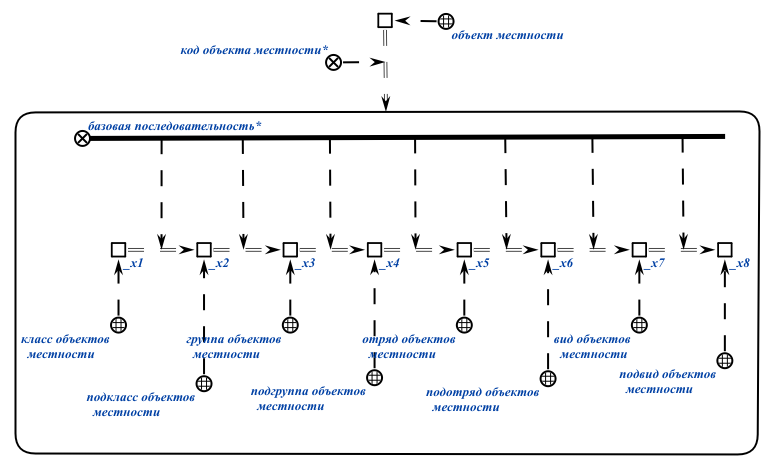
\includegraphics[scale=0.8]{author/part7/figures/geo_code.png}
\caption{Уровни иерархии классов объектов местности} 
\label{fig:pic1}
\end{figure}

Для каждого \textit{объекта местности} выделены основные, присущие только ему, семантические характеристики. Особо отметим, что метрические характеристики таким свойством не обладают.  
Согласно данному классификатору каждый класс \textit{объектов местности} имеет уникальное однозначное обозначение. Иерархия классификатора имеет восемь ступеней классификации и состоит из \textit{кода класса}, \textit{кода подкласса}, \textit{кода группы}, \textit{кода подгруппы}, \textit{кода отряда}, \textit{кода подотряда}, \textit{кода вида}, \textit{кода подвида}. Таким образом, благодаря способу кодирования уже заданы родовидовые связи, отражающие соотношения различных классов \textit{объектов местности}, а также установлены характеристики конкретного класса \textit{объектов местности}. В связи с тем, что задаются основные свойства и отношения не конкретных \textit{физических объектов}, а их классов, то такая информация является по отношению к конкретным \textit{объектам местности} метаинформацией, а совокупность данной метаинформации представляет собой онтологию \textit{объектов местности}, которая в свою очередь является частью \textit{базы знаний} \textit{интеллектуальной геоинформационной системы}.

\section{Спецификация Языка карт}
\label{chapter_gis_sec_map_specification}

\begin{SCn}
\begin{scnrelfromlist}{подраздел}
	\scnitem{\ref{chapter_gis_sec_map_syntax}~\nameref{chapter_gis_sec_map_syntax}}
	\scnitem{\ref{chapter_gis_sec_onto_model}~\nameref{chapter_gis_sec_onto_model}}
\end{scnrelfromlist}
\end{SCn}

\subsection{Синтаксис Языка карт}
\label{chapter_gis_sec_map_syntax}

\begin{SCn}	
\scnheader{объект местности}
\scnrelfrom{разбиение}{\textbf{\textit{Типология объектов местности по локализации}}\scnsupergroupsign}
\begin{scnindent}
	\begin{scneqtoset}
		\scnitem{точечный объект местности}
		\begin{scnindent}
			\scnidtf{объект местности, который не выражается в масштабе карты}
			\begin{scnrelfromlist}{пример;включение}
				\scnitem{колодец}
				\scnitem{осветительная опора}
				\scnitem{дорожный знак}
			\end{scnrelfromlist}
		\end{scnindent}
		\scnitem{линейный объект местности}
		\begin{scnindent}
			\scnidtf{объект местности, длина которого выражается в масштабе карты}
			\begin{scnrelfromlist}{пример;включение}
				\scnitem{мост}
			\end{scnrelfromlist}
		\end{scnindent}
		\scnitem{полилинейный объект местности}
		\begin{scnindent}
			\scnidtf{объект местности, состоящий из двух и более сегментов линейных объектов}
			\begin{scnrelfromlist}{пример;включение}
				\scnitem{река}
				\scnitem{дорога}
				\scnitem{улица}
			\end{scnrelfromlist}
		\end{scnindent}
		\scnitem{площадной объект местности}
		\begin{scnindent}
			\scnidtf{объект местности, площадь которого выражается в масштабе карты}
			\begin{scnrelfromlist}{пример;включение}
				\scnitem{озеро}
				\scnitem{административный район}
				\scnitem{государство}
			\end{scnrelfromlist}
		\end{scnindent}
	\end{scneqtoset}
\end{scnindent}	
\end{SCn}

Между указанными локализациями \textit{объектов местности} можно установить \textit{картографические отношения}: \textit{включение*}, \textit{граничить*}, \textit{пересечение*} и \textit{примыкание*}. 

\begin{SCn}
\scnheader{картографическое отношение}
\scnidtf{топологическое отношение}
\scnidtf{ПОЯСНИТЬ}
\scnhaselement{включение*}
\begin{scnindent}
	\scnsuperset{включение точечного объекта местности в площадной объект местности*}
	\begin{scnindent}
		\scnrelfrom{пример}{\includegraphics[scale=1.0]{author/part7/figures/point\_to\_square\_inclusion.png}}
	\end{scnindent}
	\scnsuperset{включение линейного (полилинейного) объекта местности в площадной объект местности*}
	\begin{scnindent}
		\scnrelfrom{пример}{\includegraphics[scale=1.0]{author/part7/figures/linear\_to\_square\_inclusion.png}}
	\end{scnindent}
	\scnsuperset{включение площадного объекта местности в площадной объект местности*}
	\begin{scnindent}
		\scnrelfrom{пример}{\includegraphics[scale=1.0]{author/part7/figures/square\_to\_square\_inclusion.png}}
	\end{scnindent}
\end{scnindent}
\scnhaselement{граничить*}
\begin{scnindent}
	\scnrelfrom{пример}{\includegraphics[scale=1.0]{author/part7/figures/square\_to\_square\_edgion.png}}
\end{scnindent}
\scnhaselement{пересечение*}
\begin{scnindent}
	\scnsuperset{пересечение двух линейных (полинейных) объектов местности*}
	\begin{scnindent}
		\scnrelfrom{пример}{\includegraphics[scale=1.0]{author/part7/figures/linear\_linear\_intersection.png}}
	\end{scnindent}
	\scnsuperset{пересечение линейного (полинейного) и площадного объектов местности*}
	\begin{scnindent}
		\scnrelfrom{пример}{\includegraphics[scale=1.0]{author/part7/figures/linear\_square\_intersection.png}}
	\end{scnindent}
\end{scnindent}
\scnhaselement{примыкание*}
\begin{scnindent}
	\scnrelfrom{пример}{\includegraphics[scale=1.0]{author/part7/figures/linear\_to\_linear\_contiguition.png}}
\end{scnindent}
\end{SCn}

Отношение \scnqqi{включения*} будет устанавливаться между \textit{площадным} и \textit{линейным}, \textit{площадным} и \textit{точечным}, \textit{площадными объектами местности}. Отношение \scnqqi{пересечения*} будет устанавливаться между \textit{линейными} и \textit{площадными} и \textit{линейными объектами местности}. Отношение \scnqqi{граничить*} будет устанавливаться между \textit{площадными объектами местности}. Отношение \scnqqi{примыкания*} устанавливается между \textit{линейными объектами местности}. Для всех \textit{картографических отношений} существуют структуры для их хранения.

\subsection{Денотационная семантика Языка карт}
\label{chapter_gis_sec_map_semantics}

\section{Средства автоматизации проектирования интеллектуальных геоинформационных систем}
\label{chapter_gis_sec_automatization}

%ПЕРЕСМОТРЕТЬ ВСЁ, ЧТО В КОНЦЕ
\section{Основные компоненты формальных онтологий, используемых в геоинформационных системах}

Основным подходом к обеспечению семантической интероперабельности является разработка онтологий.
Наиболее часто онтологии, используемые в геоинформатике, обычно рассматриваются как доменные онтологии, которые принято называть географическими онтологиями, или геоонтологиями (F. Fonseca, Câmara, Miguel Monteiro, 2006; Tomai  Kavouras, 2004a). 

Одной из задач в разработке онтологий является четкое и однозначное определение семантики примитивных терминов (атомарных элементов, которые не могут быть далее разделены). Чтобы решить эту проблему, исследователи предложили обосновать примитивные термины, основанные на окружающей среде и процессе наблюдения (Janowicz, 2012; Mallenby, 2007; Scheider).

\section{Гео-онтологии как подход представления информации на основе знаний}

Онтологии встраиваются в \textit{геоинформационные системы} и веб-службы
\textit{геоинформационных систем} в качестве компонента, обеспечивающего \textit{семантическую совместимость} (Frank, 1997). Проблема \textit{семантической совместимости} исследовалась FT Fonseca и Egenhofer (1999) при разработке \textit{геоинформационных систем}, основанной на онтологиях (ODGIS). В последующем, ориентированные на онтологическом инжиниринге подходы  развиты в работах Hakimpour и Timpf (2001), FT Fonseca, Egenhofer, Davis и Borges (2000), Фаллахи, Фрэнк, Месгари и Раджабифард (2008). В 2003 году Kuhn предложил к использованию семантические системы отсчета (SRS), представляющие собой основанные на онтологиях системы, аналогичные существующим пространственным и временным системам отсчета, которые получили широкое использование в \textit{геоинформационных системах} для обеспечения \textit{семантической совместимости}.
Процесс разработки онтологий называется онтологическим проектированием и согласно концепции онтологического инжиниринга онтологии должны быть разработаны, прежде чем они могут быть использованы в \textit{геоинформационных системах}. Таким образом, в основу \textit{геоинформационных систем} кладется некая \textit{предметная область}, описываемая изначально онтологической моделью. 

Из литературы можно выделить три типа онтологий: 
\begin{textitemize}
	\item онтология верхнего уровня, 
	\item онтология предметной области (доменная онтология), 
	\item шаблон проектирования онтологий (ODP).
\end{textitemize}

Онтология верхнего уровня содержит общие термины, которые можно использовать в разных предметных областях и доменах. В качестве таких терминов можно указать такие универсальные отношения как "примыкание", "пересечение", "соседство" и т.п. В работах белорусских ученых Абламейко и Крючкова () в качестве таких базовых терминов выступают пространственно-логические связи (ПЛС), а в работе (рудой в кн. абламейко 125) вводятся концептуальные топологические отношения, которые как и ПЛС являются инструментом создания топологических отношений на уровне объектов местности.  
В свою очередь онтологии предметных областей (доменные онтологии) формализуют концепции для конкретной дисциплины или предметной области  для которой проектируются ГИС. 

Наиболее часто онтологии, используемые в GIScience, обычно рассматриваются как доменные онтологии, которые принято называть  географическими онтологиями, или геоонтологиями (F. Fonseca, Câmara,  Miguel Monteiro, 2006; Tomai Kavouras, 2004a). Шаблоны проектирования онтологий разрабатываются на основе приложений. Вместо того, чтобы искать соглашения внутри или между доменами, они отражают общие потребности, разделяемые несколькими приложениями (Gangemi, 2005; Gangemi Presutti, 2009).  
Для разработки онтологий часто используются три типа подходов: нисходящий, восходящий и гибридный. 
Подходы сверху вниз опираются на инженеров знаний и экспертов в области определения и формализации онтологических концепций и отношений (Brodaric, 2004; Gates, Keller, Salayandia, Da Silva, Salcedo, 2007; Schuurman Leszczynski, 2006; Shankar, et al., 2007; Y. Wang, Gong Wu, 2007). 

Восходящие подходы используют методы интеллектуального анализа данных для извлечения понятий и отношений из структурированных баз данных или неструктурированного текста на естественном языке (Baglioni, Masserotti, Renso, Spinsanti, 2007; Buitelaar, Cimiano, Magnini, 2005; Maedche  Staab, 2004; Sen, 2007; Shamsfard Barforoush, 2004). 

Гибридные подходы объединяют предыдущие два и объединяют как экспертные знания, так и результаты процессов интеллектуального анализа данных (Buitelaar, Olejnik, Sintek, 2004; Y. Hu Janowicz, 2016; Prieto-Díaz, 2003). Одной из задач в разработке онтологий является четкое и однозначное определение семантики примитивных терминов (атомных концепций, которые не могут быть далее разделены). Чтобы решить эту проблему, исследователи предложили обосновать примитивные термины, основанные на окружающей среде и процессе наблюдения (Janowicz, 2012; Mallenby, 2007; Scheider, Janowi

Спецификация компонентов \textit{геоинформационных систем}:

\begin{figure}[H]
	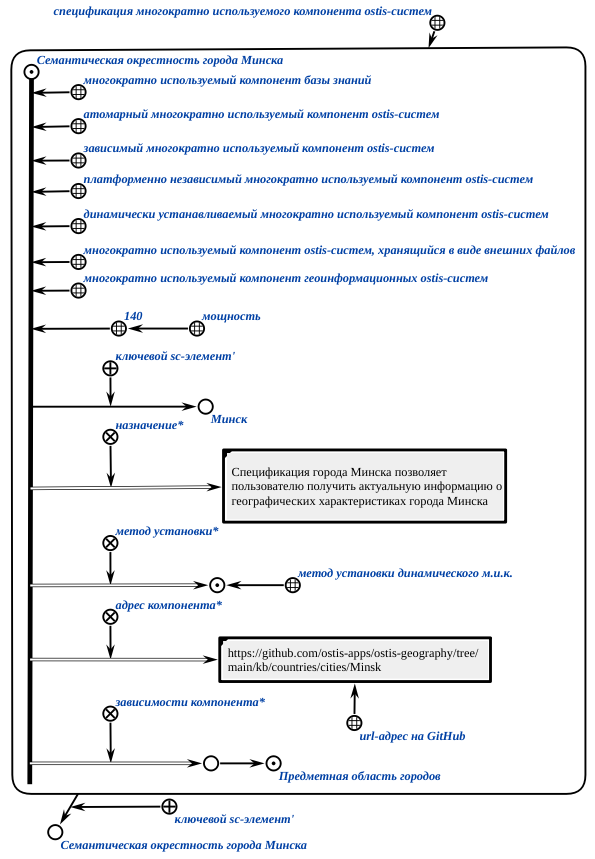
\includegraphics[scale=0.8]{author/part7/figures/gis_kb_component.png}
	\caption{Пример многократно используемого компонента базы знаний геоинформационных ostis-систем}
	\label{fig:gis_kb_component}
\end{figure}

\begin{figure}[H]
	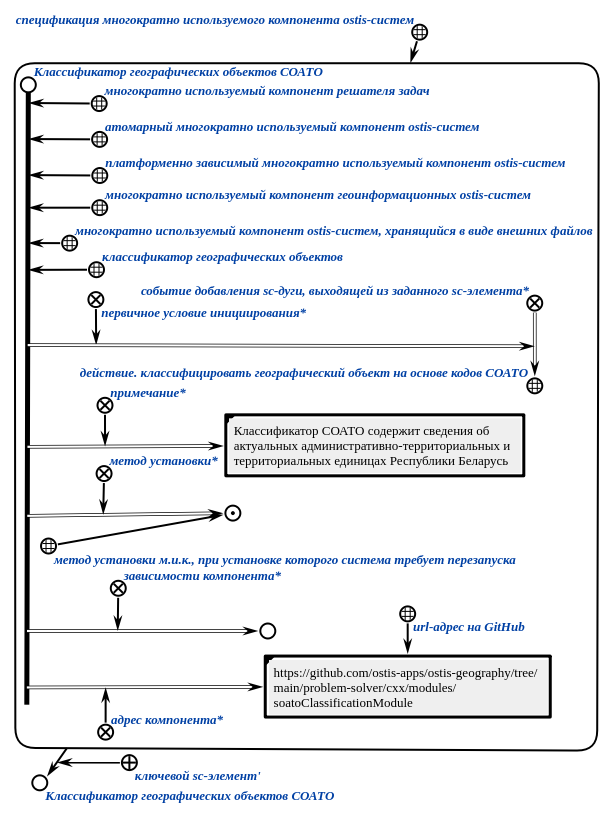
\includegraphics[scale=0.8]{author/part7/figures/gis_ps_component.png}
	\caption{Пример многократно используемого компонента решателя задач геоинформационных ostis-систем}
	\label{fig:gis_ps_component}
\end{figure}

%%%%%%%%%%%%%%%%%%%%%%%%% referenc.tex %%%%%%%%%%%%%%%%%%%%%%%%%%%%%%
% sample references
% %
% Use this file as a template for your own input.
%
%%%%%%%%%%%%%%%%%%%%%%%% Springer-Verlag %%%%%%%%%%%%%%%%%%%%%%%%%%
%
% BibTeX users please use
% \bibliographystyle{}
% \bibliography{}
%
\biblstarthook{In view of the parallel print and (chapter-wise) online publication of your book at \url{www.springerlink.com} it has been decided that -- as a genreral rule --  references should be sorted chapter-wise and placed at the end of the individual chapters. However, upon agreement with your contact at Springer you may list your references in a single seperate chapter at the end of your book. Deactivate the class option \texttt{sectrefs} and the \texttt{thebibliography} environment will be put out as a chapter of its own.\\\indent
References may be \textit{cited} in the text either by number (preferred) or by author/year.\footnote{Make sure that all references from the list are cited in the text. Those not cited should be moved to a separate \textit{Further Reading} section or chapter.} If the citatiion in the text is numbered, the reference list should be arranged in ascending order. If the citation in the text is author/year, the reference list should be \textit{sorted} alphabetically and if there are several works by the same author, the following order should be used:
\begin{enumerate}
\item all works by the author alone, ordered chronologically by year of publication
\item all works by the author with a coauthor, ordered alphabetically by coauthor
\item all works by the author with several coauthors, ordered chronologically by year of publication.
\end{enumerate}
The \textit{styling} of references\footnote{Always use the standard abbreviation of a journal's name according to the ISSN \textit{List of Title Word Abbreviations}, see \url{http://www.issn.org/en/node/344}} depends on the subject of your book:
\begin{itemize}
\item The \textit{two} recommended styles for references in books on \textit{mathematical, physical, statistical and computer sciences} are depicted in ~\cite{science-contrib, science-online, science-mono, science-journal, science-DOI} and ~\cite{phys-online, phys-mono, phys-journal, phys-DOI, phys-contrib}.
\item Examples of the most commonly used reference style in books on \textit{Psychology, Social Sciences} are~\cite{psysoc-mono, psysoc-online,psysoc-journal, psysoc-contrib, psysoc-DOI}.
\item Examples for references in books on \textit{Humanities, Linguistics, Philosophy} are~\cite{humlinphil-journal, humlinphil-contrib, humlinphil-mono, humlinphil-online, humlinphil-DOI}.
\item Examples of the basic Springer style used in publications on a wide range of subjects such as \textit{Computer Science, Economics, Engineering, Geosciences, Life Sciences, Medicine, Biomedicine} are ~\cite{basic-contrib, basic-online, basic-journal, basic-DOI, basic-mono}. 
\end{itemize}
}

\begin{thebibliography}{99.}%
% and use \bibitem to create references.
%
% Use the following syntax and markup for your references if 
% the subject of your book is from the field 
% "Mathematics, Physics, Statistics, Computer Science"
%
% Contribution 
\bibitem{science-contrib} Broy, M.: Software engineering --- from auxiliary to key technologies. In: Broy, M., Dener, E. (eds.) Software Pioneers, pp. 10-13. Springer, Heidelberg (2002)
%
% Online Document
\bibitem{science-online} Dod, J.: Effective substances. In: The Dictionary of Substances and Their Effects. Royal Society of Chemistry (1999) Available via DIALOG. \\
\url{http://www.rsc.org/dose/title of subordinate document. Cited 15 Jan 1999}
%
% Monograph
\bibitem{science-mono} Geddes, K.O., Czapor, S.R., Labahn, G.: Algorithms for Computer Algebra. Kluwer, Boston (1992) 
%
% Journal article
\bibitem{science-journal} Hamburger, C.: Quasimonotonicity, regularity and duality for nonlinear systems of partial differential equations. Ann. Mat. Pura. Appl. \textbf{169}, 321--354 (1995)
%
% Journal article by DOI
\bibitem{science-DOI} Slifka, M.K., Whitton, J.L.: Clinical implications of dysregulated cytokine production. J. Mol. Med. (2000) doi: 10.1007/s001090000086 
%
\bigskip

% Use the following (APS) syntax and markup for your references if 
% the subject of your book is from the field 
% "Mathematics, Physics, Statistics, Computer Science"
%
% Online Document
\bibitem{phys-online} J. Dod, in \textit{The Dictionary of Substances and Their Effects}, Royal Society of Chemistry. (Available via DIALOG, 1999), 
\url{http://www.rsc.org/dose/title of subordinate document. Cited 15 Jan 1999}
%
% Monograph
\bibitem{phys-mono} H. Ibach, H. L\"uth, \textit{Solid-State Physics}, 2nd edn. (Springer, New York, 1996), pp. 45-56 
%
% Journal article
\bibitem{phys-journal} S. Preuss, A. Demchuk Jr., M. Stuke, Appl. Phys. A \textbf{61}
%
% Journal article by DOI
\bibitem{phys-DOI} M.K. Slifka, J.L. Whitton, J. Mol. Med., doi: 10.1007/s001090000086
%
% Contribution 
\bibitem{phys-contrib} S.E. Smith, in \textit{Neuromuscular Junction}, ed. by E. Zaimis. Handbook of Experimental Pharmacology, vol 42 (Springer, Heidelberg, 1976), p. 593
%
\bigskip
%
% Use the following syntax and markup for your references if 
% the subject of your book is from the field 
% "Psychology, Social Sciences"
%
%
% Monograph
\bibitem{psysoc-mono} Calfee, R.~C., \& Valencia, R.~R. (1991). \textit{APA guide to preparing manuscripts for journal publication.} Washington, DC: American Psychological Association.
%
% Online Document
\bibitem{psysoc-online} Dod, J. (1999). Effective substances. In: The dictionary of substances and their effects. Royal Society of Chemistry. Available via DIALOG. \\
\url{http://www.rsc.org/dose/Effective substances.} Cited 15 Jan 1999.
%
% Journal article
\bibitem{psysoc-journal} Harris, M., Karper, E., Stacks, G., Hoffman, D., DeNiro, R., Cruz, P., et al. (2001). Writing labs and the Hollywood connection. \textit{J Film} Writing, 44(3), 213--245.
%
% Contribution 
\bibitem{psysoc-contrib} O'Neil, J.~M., \& Egan, J. (1992). Men's and women's gender role journeys: Metaphor for healing, transition, and transformation. In B.~R. Wainrig (Ed.), \textit{Gender issues across the life cycle} (pp. 107--123). New York: Springer.
%
% Journal article by DOI
\bibitem{psysoc-DOI}Kreger, M., Brindis, C.D., Manuel, D.M., Sassoubre, L. (2007). Lessons learned in systems change initiatives: benchmarks and indicators. \textit{American Journal of Community Psychology}, doi: 10.1007/s10464-007-9108-14.
%
%
% Use the following syntax and markup for your references if 
% the subject of your book is from the field 
% "Humanities, Linguistics, Philosophy"
%
\bigskip
%
% Journal article
\bibitem{humlinphil-journal} Alber John, Daniel C. O'Connell, and Sabine Kowal. 2002. Personal perspective in TV interviews. \textit{Pragmatics} 12:257--271
%
% Contribution 
\bibitem{humlinphil-contrib} Cameron, Deborah. 1997. Theoretical debates in feminist linguistics: Questions of sex and gender. In \textit{Gender and discourse}, ed. Ruth Wodak, 99--119. London: Sage Publications.
%
% Monograph
\bibitem{humlinphil-mono} Cameron, Deborah. 1985. \textit{Feminism and linguistic theory.} New York: St. Martin's Press.
%
% Online Document
\bibitem{humlinphil-online} Dod, Jake. 1999. Effective substances. In: The dictionary of substances and their effects. Royal Society of Chemistry. Available via DIALOG. \\
http://www.rsc.org/dose/title of subordinate document. Cited 15 Jan 1999
%
% Journal article by DOI
\bibitem{humlinphil-DOI} Suleiman, Camelia, Daniel C. O'Connell, and Sabine Kowal. 2002. `If you and I, if we, in this later day, lose that sacred fire...': Perspective in political interviews. \textit{Journal of Psycholinguistic Research}. doi: 10.1023/A:1015592129296.
%
%
%
\bigskip
%
%
% Use the following syntax and markup for your references if 
% the subject of your book is from the field 
% "Computer Science, Economics, Engineering, Geosciences, Life Sciences"
%
%
% Contribution 
\bibitem{basic-contrib} Brown B, Aaron M (2001) The politics of nature. In: Smith J (ed) The rise of modern genomics, 3rd edn. Wiley, New York 
%
% Online Document
\bibitem{basic-online} Dod J (1999) Effective Substances. In: The dictionary of substances and their effects. Royal Society of Chemistry. Available via DIALOG. \\
\url{http://www.rsc.org/dose/title of subordinate document. Cited 15 Jan 1999}
%
% Journal article by DOI
\bibitem{basic-DOI} Slifka MK, Whitton JL (2000) Clinical implications of dysregulated cytokine production. J Mol Med, doi: 10.1007/s001090000086
%
% Journal article
\bibitem{basic-journal} Smith J, Jones M Jr, Houghton L et al (1999) Future of health insurance. N Engl J Med 965:325--329
%
% Monograph
\bibitem{basic-mono} South J, Blass B (2001) The future of modern genomics. Blackwell, London 
%
\end{thebibliography}
